\documentclass{ximera}
\title{The development team}

\begin{document}
\begin{abstract}
  It takes quite a few people to make an experience like this possible.
\end{abstract}
\maketitle

Most of the major milestones for the Ximera Project were first met
because of the support of NSF Grant DUE-1245433; for that phase of
development, the principal investigator was Herb Clemens and Co-PIs
were Jim Fowler and Bart Snapp.

\subsection*{
\includegraphics{people/bart-snapp-150.jpg} Bart Snapp}

% 	"link":'http://www.math.osu.edu/~snapp/', 
%  "email": 'snapp.14@osu.edu'

Bart Snapp teaches mathematics at OSU.  His research interests include
commutative ring theory and recreational mathematics.  He enjoys
exploring connections between mathematics and real-world problems,
art, and music.


\subsection*{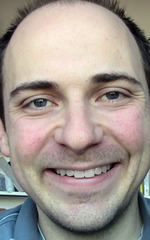
\includegraphics{people/jim-fowler-150.jpg} Jim Fowler}

% 	"link":'http://www.math.osu.edu/~fowler/',
%	"email": 'fowler@math.osu.edu'

Jim Fowler's research broadly includes geometry and topology;
specifically, his interests focus on the topology of high-dimensional
manifolds and geometric group theory, which means he thinks about
highly symmetric (and therefore very beautiful) geometric objects.
He's fond of using computational techniques to attack problems in pure
mathematics. He received an undergraduate degree from Harvard
University and received a Ph.D. from the University of Chicago.  Jim
built the adaptive learning platform that powers MOOCulus.


\end{document}

%%% Local Variables:
%%% mode: latex
%%% TeX-master: t
%%% End:
